\documentclass{article}

\usepackage{tikz} 
\usetikzlibrary{automata, positioning, arrows} 

\usepackage{amsthm}
\usepackage{amsfonts}
\usepackage{amsmath}
\usepackage{amssymb}
\usepackage{fullpage}
\usepackage{color}
\usepackage{parskip}
\usepackage{hyperref}
  \hypersetup{
    colorlinks = true,
    urlcolor = blue,       % color of external links using \href
    linkcolor= blue,       % color of internal links 
    citecolor= blue,       % color of links to bibliography
    filecolor= blue,        % color of file links
    }
    
\usepackage{listings}
\usepackage[utf8]{inputenc}                                                    
\usepackage[T1]{fontenc}   
\usepackage[margin=1in]{geometry}
\usepackage{tikz}
\usepackage{caption}
\captionsetup[figure]{labelformat=empty}
\usetikzlibrary{arrows.meta,positioning}
\tikzset{
  >=Stealth,
  obj/.style = {circle, draw, minimum size=8mm, inner sep=0pt, font=\small},
}
\newcommand{\rowlabel}[3]{\textbf{Confluent #1,\ Terminating #2,\ Unique NFs #3}}

\definecolor{dkgreen}{rgb}{0,0.6,0}
\definecolor{gray}{rgb}{0.5,0.5,0.5}
\definecolor{mauve}{rgb}{0.58,0,0.82}

\lstset{frame=tb,
  language=haskell,
  aboveskip=3mm,
  belowskip=3mm,
  showstringspaces=false,
  columns=flexible,
  basicstyle={\small\ttfamily},
  numbers=none,
  numberstyle=\tiny\color{gray},
  keywordstyle=\color{blue},
  commentstyle=\color{dkgreen},
  stringstyle=\color{mauve},
  breaklines=true,
  breakatwhitespace=true,
  tabsize=3
}

\newtheoremstyle{theorem}
  {\topsep}   % ABOVESPACE
  {\topsep}   % BELOWSPACE
  {\itshape\/}  % BODYFONT
  {0pt}       % INDENT (empty value is the same as 0pt)
  {\bfseries} % HEADFONT
  {.}         % HEADPUNCT
  {5pt plus 1pt minus 1pt} % HEADSPACE
  {}          % CUSTOM-HEAD-SPEC
\theoremstyle{theorem} 
   \newtheorem{theorem}{Theorem}[section]
   \newtheorem{corollary}[theorem]{Corollary}
   \newtheorem{lemma}[theorem]{Lemma}
   \newtheorem{proposition}[theorem]{Proposition}
\theoremstyle{definition}
   \newtheorem{definition}[theorem]{Definition}
   \newtheorem{example}[theorem]{Example}
\theoremstyle{remark}    
  \newtheorem{remark}[theorem]{Remark}

\title{CPSC-354 Report}
\author{Mitchell Toney  \\ Chapman University}

\date{\today} 

\begin{document}

\maketitle

\begin{abstract}
\end{abstract}

\setcounter{tocdepth}{3}
\tableofcontents

\section{Introduction}\label{intro}

\section{Week by Week}\label{homework}

\subsection{Week 1: HW1}
The $MU$ puzzle is a puzzle created by Douglas Hofstadter. It consists of four rules that can be applied to a string $MI$.
\[
\begin{array}{l}
1.\ xI \rightarrow xIU \\
2.\ Mx \rightarrow Mxx \\
3.\ xIIIy \rightarrow xUy \\
4.\ xUUy \rightarrow xy 
\end{array}
\]
When first approaching this puzzle, the first strategy that came to mind was to take advantage of rule number 2 to keep duplicating the I's until there is a multiple of three, then using rules 3 and 4 to get rid of the I's and leave a remaining U.

The issue with this is that $2^{n}\bmod 3$ will never equal 0, it infinitely cycles between equaling 1 and 2, and without being able to get rid of all the I's, which would require them being a multiple of 3, you will never be able to get MU.

Thus, the puzzle is not solvable.

\subsection{Week 2: HW2}


\begin{center}

% Drawing 1
\begin{minipage}{0.28\textwidth}\centering
\begin{tikzpicture}
  \draw[dashed, rounded corners] (-0.9,-0.9) rectangle (1.1,0.9);
\end{tikzpicture}
\captionof{figure}{1.\; \(A=\varnothing,\; R=\varnothing\)}
\end{minipage}\hfill
% Drawing 2
\begin{minipage}{0.28\textwidth}\centering
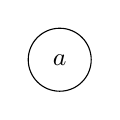
\begin{tikzpicture}
  \node[obj] (a) at (0,0) {$a$};
\end{tikzpicture}
\captionof{figure}{2.\; \(A=\{a\},\; R=\varnothing\)}
\end{minipage}\hfill
% Drawing 3
\begin{minipage}{0.28\textwidth}\centering
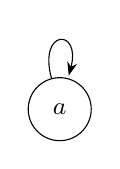
\begin{tikzpicture}
  \node[obj] (a) at (0,0) {$a$};
  \path (a) edge[loop above] (a); % (a,a)
\end{tikzpicture}
\captionof{figure}{3.\; \(A=\{a\},\; R=\{(a,a)\}\)}
\end{minipage}

\vspace{1em}

% Drawing 4
\begin{minipage}{0.28\textwidth}\centering
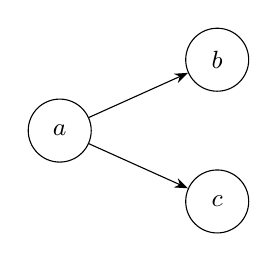
\begin{tikzpicture}
  \node[obj] (a) at (0,0) {$a$};
  \node[obj] (b) at (2,0.9) {$b$};
  \node[obj] (c) at (2,-0.9) {$c$};
  \draw[->] (a) -- (b);  % (a,b)
  \draw[->] (a) -- (c);  % (a,c)
\end{tikzpicture}
\captionof{figure}{4.\; \(A=\{a,b,c\},\; R=\{(a,b),(a,c)\}\)}
\end{minipage}\hfill
% Drawing 5
\begin{minipage}{0.28\textwidth}\centering
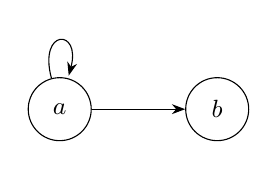
\begin{tikzpicture}
  \node[obj] (a) at (0,0) {$a$};
  \node[obj] (b) at (2,0) {$b$};
  \path (a) edge[loop above] (a); % (a,a)
  \draw[->] (a) -- (b);          % (a,b)
\end{tikzpicture}
\captionof{figure}{5.\; \(A=\{a,b\},\; R=\{(a,a),(a,b)\}\)}
\end{minipage}\hfill
% Drawing 6
\begin{minipage}{0.28\textwidth}\centering
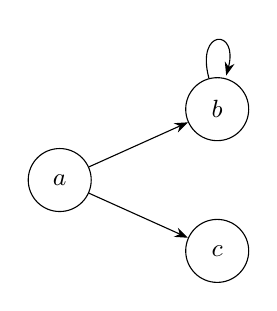
\begin{tikzpicture}
  \node[obj] (a) at (0,0) {$a$};
  \node[obj] (b) at (2,0.9) {$b$};
  \node[obj] (c) at (2,-0.9) {$c$};
  \draw[->] (a) -- (b);       % (a,b)
  \draw[->] (a) -- (c);       % (a,c)
  \path (b) edge[loop above] (b); % (b,b)
\end{tikzpicture}
\captionof{figure}{6.\; \(A=\{a,b,c\},\; R=\{(a,b),(b,b),(a,c)\}\)}
\end{minipage}

\vspace{1em}

% Drawing 7
\begin{minipage}{0.28\textwidth}\centering
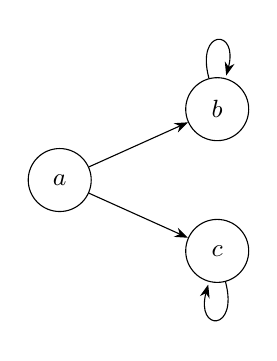
\begin{tikzpicture}
  \node[obj] (a) at (0,0) {$a$};
  \node[obj] (b) at (2,0.9) {$b$};
  \node[obj] (c) at (2,-0.9) {$c$};
  \draw[->] (a) -- (b);            % (a,b)
  \draw[->] (a) -- (c);            % (a,c)
  \path (b) edge[loop above] (b);  % (b,b)
  \path (c) edge[loop below] (c);  % (c,c)
\end{tikzpicture}
\captionof{figure}{7.\; \(A=\{a,b,c\},\; R=\{(a,b),(b,b),(a,c),(c,c)\}\)}
\end{minipage}

\end{center}

\[
\begin{array}{c|c|c|c}
\text{\#} & \text{Terminating} & \text{Confluent} & \text{Unique NFs}\\\hline
1 & \text{Yes} & \text{Yes} & \text{Yes}\\
2 & \text{Yes} & \text{Yes} & \text{Yes}\\
3 & \text{No}  & \text{Yes} & \text{No}\\
4 & \text{Yes} & \text{No}  & \text{No}\\
5 & \text{No}  & \text{Yes} & \text{Yes}\\
6 & \text{No}  & \text{No}  & \text{No}\\
7 & \text{No}  & \text{No}  & \text{No}
\end{array}
\]

\noindent\rule{\textwidth}{0.4pt}

\begin{center}

% Row 1
\begin{minipage}{0.45\textwidth}\centering
\rowlabel{True}{True}{True}\par\vspace{0.35em}
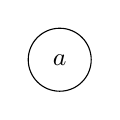
\begin{tikzpicture}
  \node[obj] (a) at (0,0) {$a$};
\end{tikzpicture}

$A=\{a\},\ R=\varnothing$
\end{minipage}\hfill
% Row 2
\begin{minipage}{0.45\textwidth}\centering
\rowlabel{True}{True}{False}\par\vspace{0.35em}
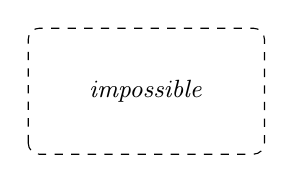
\begin{tikzpicture}
  \draw[dashed, rounded corners] (-1.5,-0.8) rectangle (1.5,0.8);
  \node at (0,0) {\small \emph{impossible}};
\end{tikzpicture}

(no ARS exists)
\end{minipage}

\vspace{1.2em}

% Row 3
\begin{minipage}{0.45\textwidth}\centering
\rowlabel{True}{False}{True}\par\vspace{0.35em}
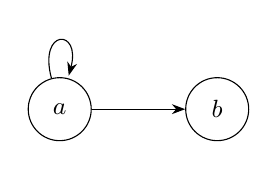
\begin{tikzpicture}
  \node[obj] (a) at (0,0) {$a$};
  \node[obj] (b) at (2,0) {$b$};
  \path (a) edge[loop above] (a);
  \draw[->] (a) -- (b);
\end{tikzpicture}

$A=\{a,b\},\ R=\{(a,a),(a,b)\}$
\end{minipage}\hfill
% Row 4
\begin{minipage}{0.45\textwidth}\centering
\rowlabel{True}{False}{False}\par\vspace{0.35em}
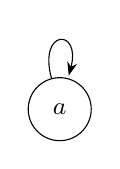
\begin{tikzpicture}
  \node[obj] (a) at (0,0) {$a$};
  \path (a) edge[loop above] (a);
\end{tikzpicture}

$A=\{a\},\ R=\{(a,a)\}$
\end{minipage}

\vspace{1.2em}

% Row 5
\begin{minipage}{0.45\textwidth}\centering
\rowlabel{False}{True}{True}\par\vspace{0.35em}
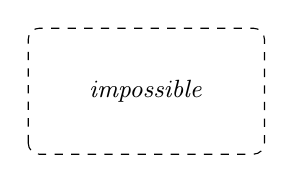
\begin{tikzpicture}
  \draw[dashed, rounded corners] (-1.5,-0.8) rectangle (1.5,0.8);
  \node at (0,0) {\small \emph{impossible}};
\end{tikzpicture}

(no ARS exists)
\end{minipage}\hfill
% Row 6
\begin{minipage}{0.45\textwidth}\centering
\rowlabel{False}{True}{False}\par\vspace{0.35em}
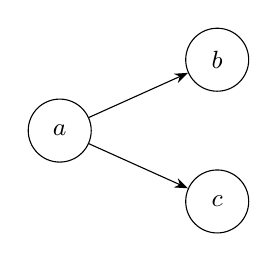
\begin{tikzpicture}
  \node[obj] (a) at (0,0) {$a$};
  \node[obj] (b) at (2,0.9) {$b$};
  \node[obj] (c) at (2,-0.9) {$c$};
  \draw[->] (a) -- (b);
  \draw[->] (a) -- (c);
\end{tikzpicture}

$A=\{a,b,c\},\ R=\{(a,b),(a,c)\}$
\end{minipage}

\vspace{1.2em}

% Row 7
\begin{minipage}{0.45\textwidth}\centering
\rowlabel{False}{False}{True}\par\vspace{0.35em}
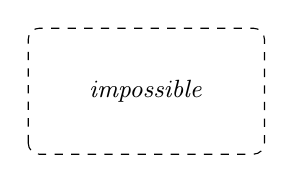
\begin{tikzpicture}
  \draw[dashed, rounded corners] (-1.5,-0.8) rectangle (1.5,0.8);
  \node at (0,0) {\small \emph{impossible}};
\end{tikzpicture}

(no ARS exists)
\end{minipage}\hfill
% Row 8
\begin{minipage}{0.45\textwidth}\centering
\rowlabel{False}{False}{False}\par\vspace{0.35em}
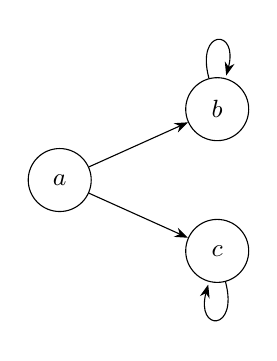
\begin{tikzpicture}
  \node[obj] (a) at (0,0) {$a$};
  \node[obj] (b) at (2,0.9) {$b$};
  \node[obj] (c) at (2,-0.9) {$c$};
  \draw[->] (a) -- (b);
  \draw[->] (a) -- (c);
  \path (b) edge[loop above] (b);
  \path (c) edge[loop below] (c);
\end{tikzpicture}

$A=\{a,b,c\},\ R=\{(a,b),(a,c),(b,b),(c,c)\}$
\end{minipage}

\end{center}

\section{Essay}

\section{Evidence of Participation}

\section{Conclusion}\label{conclusion}

\begin{thebibliography}{99}
\bibitem[BLA]{bla} Author, \href{https://en.wikipedia.org/wiki/LaTeX}{Title}, Publisher, Year.
\end{thebibliography}

\end{document}
